\lecture{13}{11 Mar 2025}{10:10}
\section{Lagrange Interpolation Proof}
\begin{proof}
    The Lagnrange polynomial \(L_{nk} (x) \) is given as 
    \[
        L_{nk}(x) = 
        \prod_{i=0, i\neq  k}^n \frac{x-x_i}{x_k - x_i} 
    \]
    If \(L_{nk} (x_j) = \delta_{kj} \) then if \(k=j\) the whole expression cancels to be one. And \(0\) if otherwise. 
    Let us now show that 
    \[
        P(x_j) = \sum_{k=0}^{n} f(x_k)L_{nk} (x_j) = f(x_j), \quad 0 \leq  j \leq n
    \]
    which we can do easily. Since \(P(x)\) passes through all nodes, it must be a unique answer since for a function s.t 
    \(Q(x_j) = y_j\) must be that \(P(x_j)-Q(x_j)\) which implies uniqueness. Since both are \(n\) degree,
    by the fundamental theorem of algebra it must be that with \(n \) real roots they are the same. 
\end{proof}
\begin{eg}
    Below are examples of graphs generated by Lagrange Interpolation
\begin{figure}[H]
    \centering
    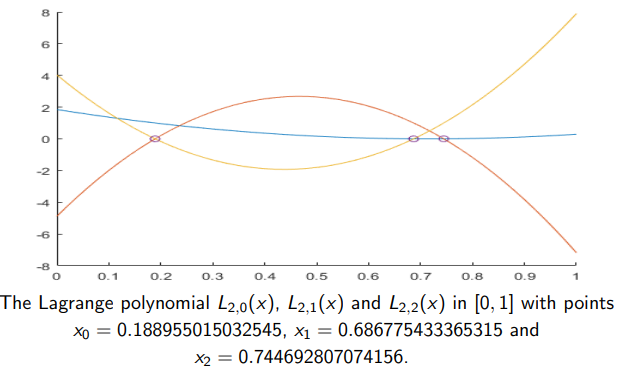
\includegraphics[width=0.6\textwidth]{Figures/01.png}
    \caption{}
    \label{fig:}
\end{figure}
\begin{figure}[H]
    \centering
    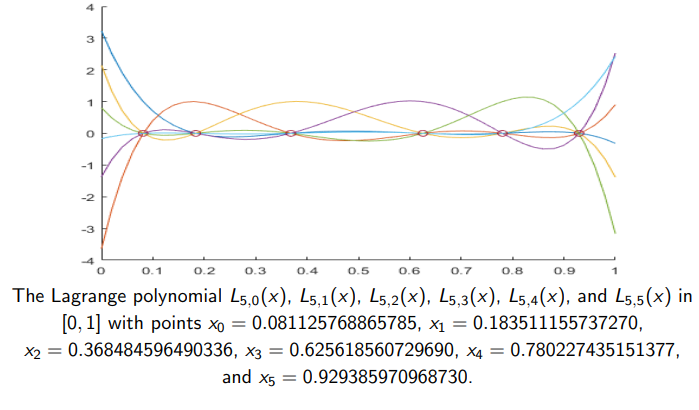
\includegraphics[width=0.6\textwidth]{Figures/02.png}
    \caption{}
    \label{fig:}
\end{figure}
\end{eg}

\begin{remark}
    Lagrange interpolation is an explicit formula without any additional computation. For example, a interpolation from two points
    has the form 
    \[
        P_1 (x) = p_0 + p_1 x
    \]
    \[
        P_1(x) = y_0 \frac{y_1 y_0}{x_1 - x_0} (x- x_0)
    \]
\end{remark}

\section{Hermite Interpolation}
\begin{definition}
    Osculatory Polynomial Approximation: Suppose we had \(n+1\) distinct points on a closed interval with a set of \(n+1\) arbitrary integers taking
    \(m \equiv \max (m_0,m_1, \dots ,m_n)\) . The osculating polynomial approximation is a polynomial \(P(x)\) s.t. 
    \[
        \frac{\mathrm{d}^{k_i} P}{\mathrm{d}x^{k_i}} (x_i) = 
        \frac{\mathrm{d}^{k_i} f}{\mathrm{d}x^{k_i}}(x_i) , \quad \forall 0 \leq  k_i \leq  m
    \]
\end{definition}
We can understand two approximations: taylor and lagrange polynomial approximation where Taylor is given by 
\[
    P(x) = \sum_{k=0}^{m_0} \frac{f^(k)(x_0)}{k!}(x-x_{0} )^k
\]
For the taylor apprixmation, we are matching the derivatives of the function \(f\) to an order up to \(m_0\) at \(x_0\). For the 
Lagrange approximation we are matching all \(n+1\) function values rather the values of the derivatives. 
\begin{definition}
    Hermite Approximation: When \(m_i = 1\)  for all \(0 \leq  i \leq  n\) we wish to match the function values there 
    as well as the first derivatives such that 
    \[
        P(x_i) = f(x_i), \quad P^{\prime} (x_i) = f^{\prime} (x_i)
    \]
\end{definition}    

\begin{theorem}
    Let \(f \in \mathcal{C}^1\) with points. There exists a unique polynomial that it matches the Hermite Approximation conditions with a degree 
    of at most \(2n+1\) where
    \[
        H_{2n+1}  (x) = \sum_{j=0}^{n} f(x_j) H_j(x) + \sum_{j=0}^{n} f^{\prime} (x_j) \hat{H} _j (x)
    \]
    where 
    \[
        H_j(x) = \left[  1- 2(x-x_j)L^{\prime}_{nj} (x_j) \right] L^{2}_{nj} (x), \quad
        \hat{H} _j(x) = (x- x_j)L^{2}_{nj} (x)
    \]
\end{theorem}
\begin{theorem}
    If \(f \in C^{2n+2} \) then 
    \[
        f(x) = H_{2n+1}(x) + 
        \frac{f^{(2n+2)} (\zeta)}{(2n+2)!} \prod_{i=0}^n (x-x_i)^{2}  
    \]
\end{theorem}